\documentclass{./../Latex/handout}
\begin{document}
\thispagestyle{plain}
\newcommand{\mytitle}{Exponential and Logarithmic Functions}
\myheader{\mytitle}

\textit{Reference:} Chiang, Alpha C, and Wainwright K. (2005), Fundamental Methods of Mathematical Economics: 4th edition, Chapter 10 

Exponential and logarithmic functions have important applications in economics. So we will discuss some basic properties and derivatives for these functions.

\section{Exponential Functions}
The exponential or power function can be represented as:
$$
y=f(t)=b^{t} \quad(b>1)
$$
where $b$ denotes a fixed base of the exponent. Note that $y$ is a function of $t$, i.e. the power of $b$. A more generalized version can be written as:
$$
y=a b^{c t}
$$ 
When the base is a special mathematical constant called Euler's number $e=2.71828...$, i.e.
$$
y=a e^{r t}
$$
it is referred to as the natural exponential function (though common to just refer to it as the exponential function as most other exponential functions don't show up as often). It is also common to write it as:
$$
y=a \exp (r t)
$$ 

Where did this number $e$ come from? It can be shown that:
$$
e \equiv \lim _{n \rightarrow \infty}\left(1+\frac{1}{n}\right)^{n}
$$
Jacob Bernoulli discovered this constant in 1683 while studying a question about compound interest. 

Suppose you invest A dollars at a 5\% interest rate that compounds yearly. After one year you will have:
\[ A \left(1+0.05\right)  \] 
After $t$ years:
\[ A \left(1+0.05\right)^{t} \]
Now rewrite the expression above as:
\[ A\left( \underbrace{\left(1+\frac{1}{1/0.05}\right)^{1/0.05}}_{\approx e} \right)^{0.05t} \approx A e^{0.05t}  \]
More generally, if $A$ is the initial principal, $r$ is the interest rate, and $t$ is the investment horizon, then the principal at $t$:
$$ A_t \approx A_0 e^{rt} $$

\section{Logarithmic Functions}
Since the exponential function is a monotonic function, its inverse exists. The inverse of the exponential function is called the log or logarithmic function.

For the exponential function: 
\[ y=b^{t} \rightarrow log_b(y) = t  \]
where the expression on the right-hand side is referred to as the $log$ of $y$ to base $b$. For the natural exponential function:
\[y=e^{t} \rightarrow \log _{e} y =ln(y) \]

Since the natural log is employed quite often, we can write it without the base as $ln$. If you say log of $x$, without mentioning the base, it is sort of assumed that you are talking about the natural log. 

For example, since $2^{3}=8$. So we can write $\log _{3} 8=2$. 

Since $y=b^{t} \Longleftrightarrow t=\log _{b} y$, we can write
$$
b^{\log _{b} y}=b^{t}=y
$$

Figure 1 presents plots for $y = e^x = exp(x)$ and $y=ln(x)$. From the plots, we can see that both log and exponential functions are strictly monotonically increasing. In addition,
\begin{itemize}
	\item $y=1$, $log(y) = 0$
	\item $0<y<1$,  $\log y<0$
	\item $\log y \rightarrow \infty$ as $y \rightarrow \infty$
	\item $\log y \rightarrow-\infty$ as $y \rightarrow 0$
\end{itemize}


\pgfplotsset{%
    width=8cm,
    height=7cm
}
\begin{figure*}[t]
\begin{subfigure}[b]{0.5\textwidth}
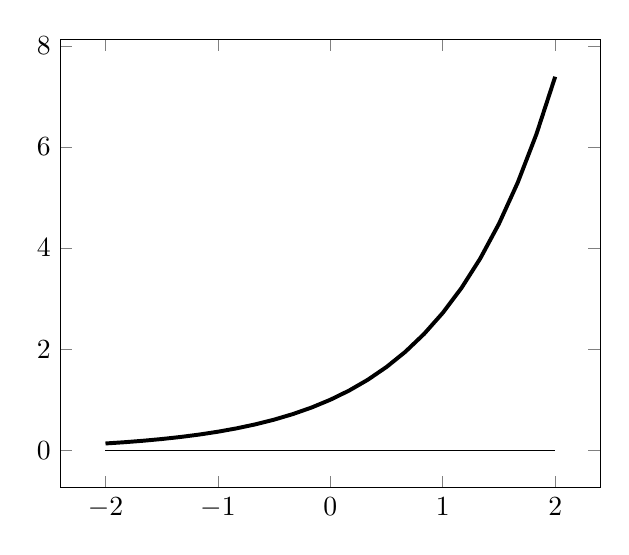
\begin{tikzpicture}
\begin{axis}[]
\addplot[color=black, line width=0.5mm, domain=-2:2] {exp(x)};
\addplot[domain=-2:2] {0};
\end{axis}
\end{tikzpicture} 
\caption{$y = e^x$}
\end{subfigure}
\begin{subfigure}[b]{0.5\textwidth}
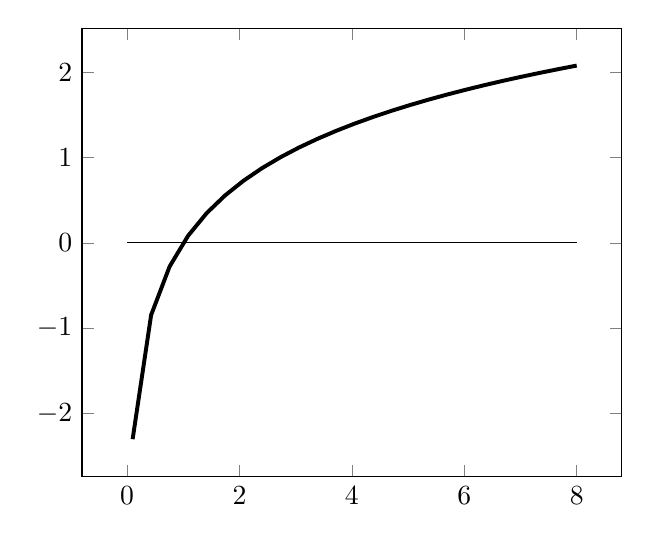
\begin{tikzpicture}
\begin{axis}[]
\addplot[color=black, line width=0.5mm, domain=0.1:8] {ln(x)};
\addplot[domain=0:8] {0};
\end{axis}
\end{tikzpicture} 
\caption{$y =ln(x)$}
\end{subfigure}
\caption{Plots for exponential and logarithmic functions}
\end{figure*}


\section{Rules for Logarithmic Functions}
\begin{itemize}
	\item $\ln (u v)=\ln u+\ln v$ 
	\item $\ln (u / v)=\ln u-\ln v$
	\item $\ln u^{a}=a \ln u$
\end{itemize}

To see why the above rules hold, let $\ln u = s$ and $\ln v = t$. Then, $u=e^s$ and $v=e^t$. In which case,
\[ uv = e^s e^t = e^{s+t} \rightarrow \ln uv =s+t = \ln u + \ln v \]
Similarly, 
\[ u/v = e^s/e^t = e^{s-t} \rightarrow \ln (u/v) =s-t = \ln u - \ln v \]
Finally for the last rule, 
\[u^a = (e^s)^a=e^{as} \rightarrow \ln u^a = as = a\ln u \]

\section{Derivatives of Exponential and Logarithmic Functions}
Derivative of the exponential function:
\[ y=b^{t} \quad \rightarrow \quad \frac{dy}{dt} = b^t \ln b  \]

Derivative of the natural exponential function:
$$ y=e^t \quad \rightarrow \quad \frac{dy}{dt} = e^t $$
Then by chain rule:
 $$y=e^{f(t)} \quad \rightarrow \quad \frac{dy}{dt} = f'(t) e^{f(t)}$$
 Derivative of the log function:
 $$ \frac{d}{d t} \ln t =\frac{1}{t} $$ \\
 Then by chain rule:
 $$ \frac{d}{d t} \ln f(t) =\frac{f'(t)}{f(t)} $$ \\
 
\textit{Let's find the derivatives for the following functions:}
\begin{enumerate}
\item $f(t)=e^t$, $f'(t) = e^t$
\item $f(t)=\ln t$, $f'(t) = 1/t$
\item $f(t)=ae^{rt}$, $f'(t) = are^{rt}$
\item $f(t)=e^{-t}$, $f'(t) = -e^{-t}$
\item $f(t)=\ln a t$, $f'(t) = a/at = 1/t$
\item $f(t)=\ln t^{c}$, $f'(t) = ct^{c-1}/t^c = c/t$
\end{enumerate}


\end{document}